\section{Proximal Policy Optimization (PPO) Algorithm}


Reinforcement Learning (RL) spans a wide range of algorithms designed to enable an agent to learn optimal behavior through interactions with its environment. This interaction is formally modeled as a Markov Decision Process (MDP) represented by the tuple $(\mathcal{S}, \mathcal{A}, P, R, \gamma)$. Here, $\mathcal{S}$ denotes the set of all possible states of the environment (such as the sailboat's position, CMG, and wind angle), while $\mathcal{A}$ represents the set of all possible actions (such as turn left, turn right or maintain heading rudder via rudder corrections). The transition dynamics are encoded by the probability function $P(s'|s,a)$, which gives the likelihood of reaching state $s'$ after taking action $a$ in state $s$. The scalar reward function $R(s,a)$ provides feedback on the quality of actions (such as CMG). Finally, the discount factor $\gamma \in [0,1]$ balances the importance of immediate versus future rewards guiding the agent toward long term optimal behavior.

\begin{figure}[H]
    \centering
    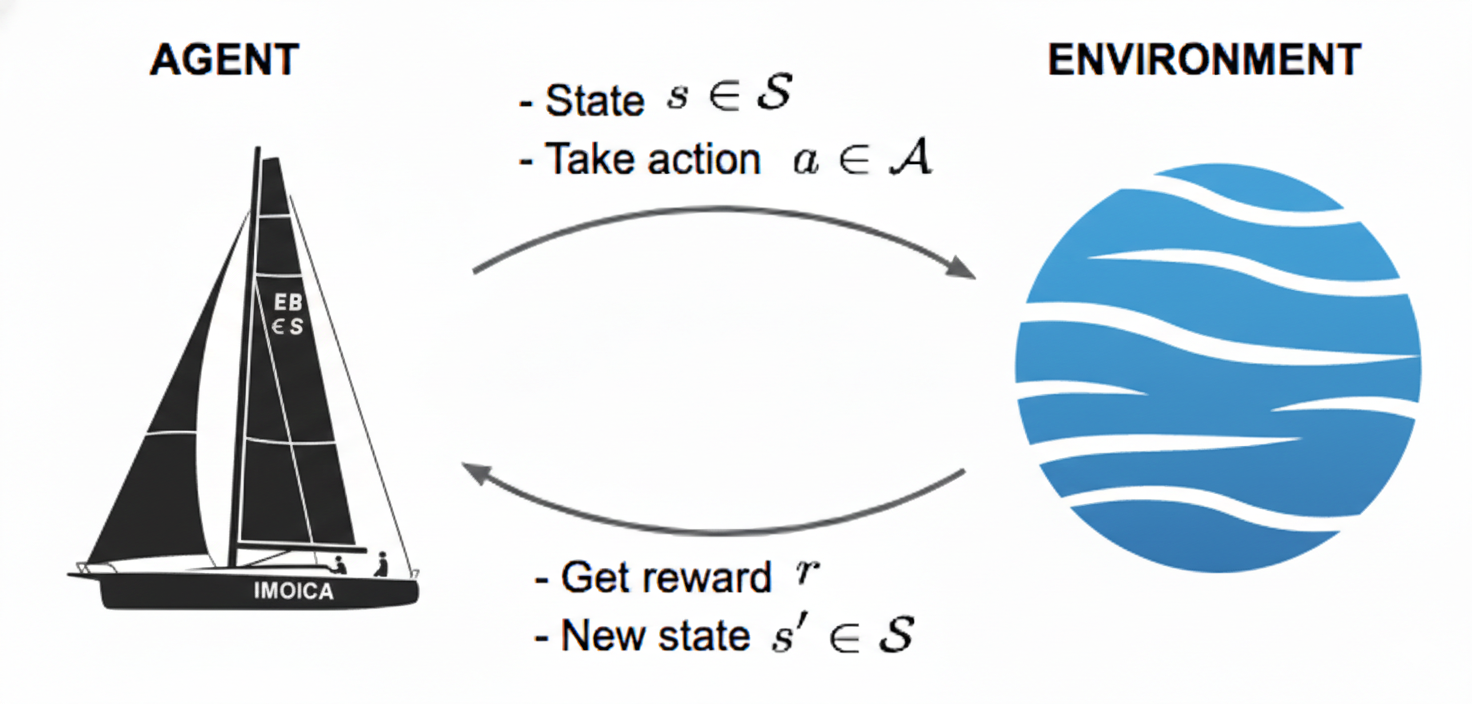
\includegraphics[width=0.6\linewidth]{resources/img/Gemini_Generated_Image_rhs7gfrhs7gfrhs7.png}
    \caption{ Markov Decision Process (MDP) of Reinforcement Learning}
    \label{fig:placeholder}
\end{figure}

\justify A \textbf{policy}, denoted as $\pi(a|s)$, is a mapping from states to a probability distribution over actions. It encodes the agent's behavior: given a state $s$, the policy defines the likelihood of taking each possible action $a$. The objective of RL is to learn an optimal policy $\pi^*$ that maximizes the expected cumulative reward over time:

\begin{equation}
J(\pi) = \mathbb{E}_{\tau \sim \pi} \Bigg[ \sum_{t=0}^{T} \gamma^t r(s_t, a_t) \Bigg],
\end{equation}

where $\tau = (s_0, a_0, s_1, a_1, \dots)$ denotes a trajectory generated by following policy $\pi$.

\justify To optimize this objective, \textbf{Policy Gradient methods} directly parameterize the policy and update it to increase the probability of actions that yield a high advantage (performing better than average). This approach is naturally suited for continuous action spaces and stochastic policies.



\subsection{From Policy Gradients to PPO}

\justify Vanilla policy gradient methods can be unstable due to large parameter updates. Trust region methods such as TRPO stabilize learning by constraining policy updates within a KL-divergence-based region, but they require complex second-order optimization. PPO simplifies this approach by introducing a \emph{clipped surrogate objective} that constrains the update magnitude while remaining compatible with first-order optimization.  

\justify In PPO, a probability ratio is defined between the new policy $\pi_\theta$ and the old policy $\pi_{\theta_\text{old}}$:

\begin{equation}
r_t(\theta) = \frac{\pi_\theta(a_t|s_t)}{\pi_{\theta_\text{old}}(a_t|s_t)}.
\end{equation}

The clipped objective is then:

\begin{equation}
L^\text{CLIP}(\theta) = \mathbb{E}_t \Big[ \min \big( r_t(\theta) A_t, \ \text{clip}(r_t(\theta), 1-\epsilon, 1+\epsilon) A_t \big) \Big],
\end{equation}

where $\epsilon$ (e.g., 0.2) sets the clipping threshold, and \(A_t\) is estimated by GAE. This objective ensures that updates do not move the policy too far in a single step, providing a “pessimistic” lower bound: policy changes that would improve the objective beyond the threshold are ignored, while detrimental changes are penalized.



\subsection{Hyperparameter Selection and Adaptation for Sailboat Navigation}
\label{sec:hyp}
\justify PPO performance is sensitive to several hyperparameters. The rollout horizon $T$ defines the number of steps over which the agent collects experience before updating the policy. While canonical papers use $T=2048$ for complex robotics tasks, we selected $T=128$ steps (corresponding to 60 seconds) to ensure frequent updates that can respond effectively to rapidly changing wind and wave conditions. The discount factor $\gamma$ balances immediate versus delayed rewards; with $\gamma=0.995$, the agent accounts for the delayed effect of rudder inputs on CMG, preventing shortsighted behavior. To reduce variance in noisy environments, the Generalized Advantage Estimator (GAE) parameter $\lambda$ was set to 0.92, slightly lower than the typical 0.95 in robotics benchmarks, which helps smooth high-frequency fluctuations from waves while capturing the underlying navigation strategy. The clipping parameter $\epsilon=0.2$ ensures that policy updates remain within a safe "trust region," preventing large, destabilizing changes when sudden wind gusts occur. A linearly decayed learning rate from $10^{-3}$ to $10^{-5}$ allows the agent to first learn basic sailing dynamics before fine-tuning maneuvers for optimal CMG. Exploration is encouraged through an entropy bonus $c_2 = 0.01$, preventing the agent from settling into sub-optimal, overly conservative rudder strategies. Finally, the neural network architecture employs a lightweight $64 \times 64$ MLP, providing sufficient capacity for learning the mapping from environmental states to actions while remaining compatible with real-time control at 2 Hz. Overall, these adaptations reflect a careful balance between literature-recommended defaults and the unique dynamics and stochasticity of autonomous sailboat navigation.
